\documentclass[11pt,a4paper]{report}
\usepackage[utf8]{inputenc}
\usepackage{amsmath}
\usepackage{amsfonts}
\usepackage{amssymb}
\usepackage{graphicx}
\author{Ryan Lance}
\title{HWK 1}
\begin{document}

\paragraph{Capstones: Classical Mechanics, HWK 1.} Ryan Lance
\paragraph{Problem 1} A cannon shoots a ball with elevation angle (the angle from the horizontal) $\theta$ and initial speed $v_o$. Ignoring air friction, find the equation of motion of the ball in the horizontal direction $(x(t))$, in the vertical direction $(y(t))$, and eliminate time to find $y(x)$. Assume that the size of the cannonball is negligible.
\paragraph{Solution} Below is a picture of the problem. One assumption is that we are only concerned with the trajectory of the cannonball immediately after it leaves the barrel of the cannon, which is stationed at $(x_o, y_o)$. The cannon is angled at angle theta with respect to the ground, and the velocity of the cannonball as it leaves the cannon is $v_o$. 

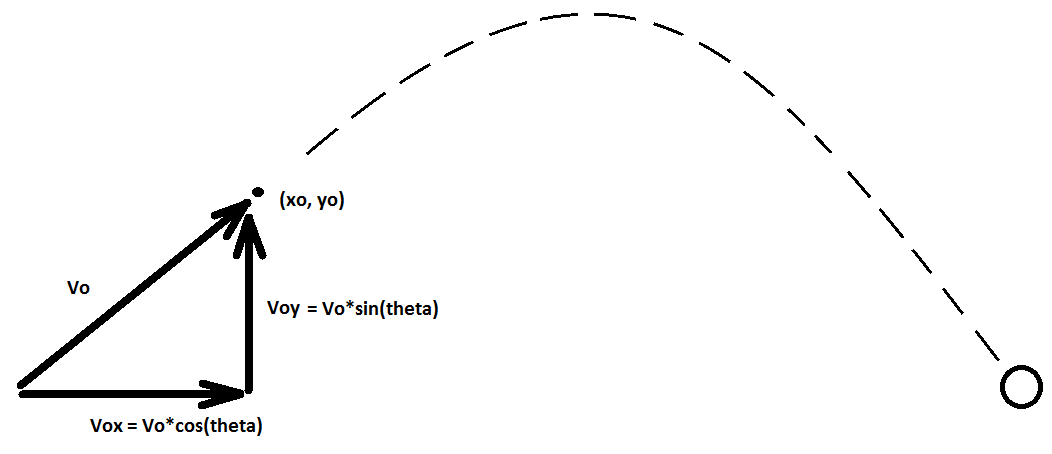
\includegraphics[scale=0.4]{pic1}
\paragraph{} We can start by splitting our velocity vector into two components $V_{ox}$ and $V_{oy}$ using sine and cosine. This way we can describe the horizontal and vertical components independently. Since our vertical axis is aligned with the gravitational field, and the cannonball is likely not going to travel very high or far, we can assume that the acceleration in the y-axis is a constant $g$ equal to $-9.81m/s^2$ and that the horizontal component of the acceleration is zero (because there is no drag). 

\paragraph{}First, we write down the acceleration component wise, then integrate with respect to time to find to find functions for velocity and position. The constants of integration become $v_{ox}, v_{oy}, x_o,$ and $y_o$.
\begin{center}
\begin{tabular}{l l}
$a_x(t) = 0$ 				& $a_y(t) = g$ \\
$v_x(t) = v_{ox}$ 			& $v_y(t) = gt + v_{oy}$ \\
$x(t) = v_{ox}t + x_o$ 		& $y(t) = 0.5gt^2 + v_{oy}t + y_o$ \\
\end{tabular}
\end{center}
\paragraph{}We now have equations for $x(t)$ and $y(t)$, but they are not in terms of $v_o$ and $\theta$. Substituting the following from earlier: $v_{ox} = v_osin(\theta), v_{oy} = v_ocos(\theta)$, and set $x_o = y_o = 0$. 
\begin{center}
\begin{tabular}{l}
$x(t) = v_ocos(\theta)t$ \\ $y(t) = 0.5gt^2 + v_osin(\theta)t$ \\
\end{tabular}
\end{center}
\paragraph{}Solving for $t$ (now $x(t) = x$), we get a formula for time in terms of $x$:
$$t = \frac{x}{v_ocos(\theta)}$$
\paragraph{}Substituting this into our equation describing vertical motion $(y(t))$ we get a new function $y(x)$ that we were looking for:
$$y(x) = 0.5g(\frac{x}{v_ocos(\theta)})^2 + v_osin(\theta)(\frac{x}{v_ocos(\theta)})$$
\paragraph{}Simplification:
$$y(x) = \frac{gx^2}{2(v_ocos(\theta))^2} + xtan(\theta)$$
\paragraph{Physical Reasoning} My physical intuition tells me that for some $\theta$ between $0$ and $\pi/2$, the motion should be a downward parabola beginning at $(x_o, y_o)$ (which is $(0, 0)$ in this case). Our solution takes the form: $ax^2 + bx$ where $a$ is negative because $g$ is negative and the denominator is squared. If we just look at $a$, we can see that it represents how quickly the trajectory will lead the cannonball back to $y = 0$. $a$ scales up with $g$ and it scales down with $v_o$. This makes sense because lower gravity or a larger initial velocity will shoot the cannonball higher and farther. Looking at the coefficient to the linear component, $tan(\theta)$, we see that at $\theta = 0$ the cannonball goes nowhere. When $\theta$ gets closer to $pi/2$ however, $tan(\theta)$ is much larger. This makes the parabola very "spiky", the cannonball is just shot up and straight down. Interestingly, this term also makes sense because when $\theta$ does go to $\pi/2$, the solution is undefined (a vertical line), which is what we expect the cannonball's path to be if the cannon is pointing straight up.

\paragraph{Problem 2} A brick, starting from rest, slides down an incline with kinetic friction coefficient $u_k$. Find the velocity of the brick when it hits the ground as a function of the angle $\theta$ that the plane makes with the horizontal and of the initial elevation $h$ of the brick from the ground. How much energy was dissipated into heat? Assume that the size of the brick is negligible.


\end{document}
